\subsection*{Tábor - co a jak, ale z jiné stránky ;)} % (fold)
\label{ssub:tábor_co_a_jak}


Možná že někteří tuší, někteří netuší a někteří třeba i ví. Naše Keyácké souoddílí čas od času mění tábořiště, přesněji řečeno přibližně jednou za dva roky. Nemáme totiž žádné trvalé tábořiště. A vlastně ho ani nechceme.
Přece jenom, střídání tábořišť má takové svoje kouzlo… 
Ale taky to s sebou nese mnoho práce s nalezením vhodného místa k táboření (tak, aby tam například už nebyl nějaký jiný tábor).

Pojďme se na ten tábor podívat s širšího pohledu: takhle nějak se tábor chová v průběhu roku: \\
\textbf{Září:}

Prázdniny jsou pryč a je čas všechno začít postupně řešit. Tady se vybírá úderný tým několika uďů, kteří budou mít místo k táboření pod palcem.\\
\textbf{Říjen:}

Zvolený tým se schází a začíná první fáze hledání vhodné louky. To znamená prohlížení map a satelitních snímků, hodnocení různých kritérií a následný výběr těch nejlepších luk.

Následně se svolává výjezd a pár uďů se jede na louku podívat, například zhodnotit stav potoka a lesa.\\
\textbf{Listopad:}

Výjezdy ještě pokračují. Obvykle bývají přibližně dva až čtyři v průběhu jednoho hledání tábořiště.
Když se podaří najít vhodnou louku, svolává se další porada, která má za cíl zjistit kdo louku vlastní a jestli nám tam v létě dovolí tábořit.
\begin{center}
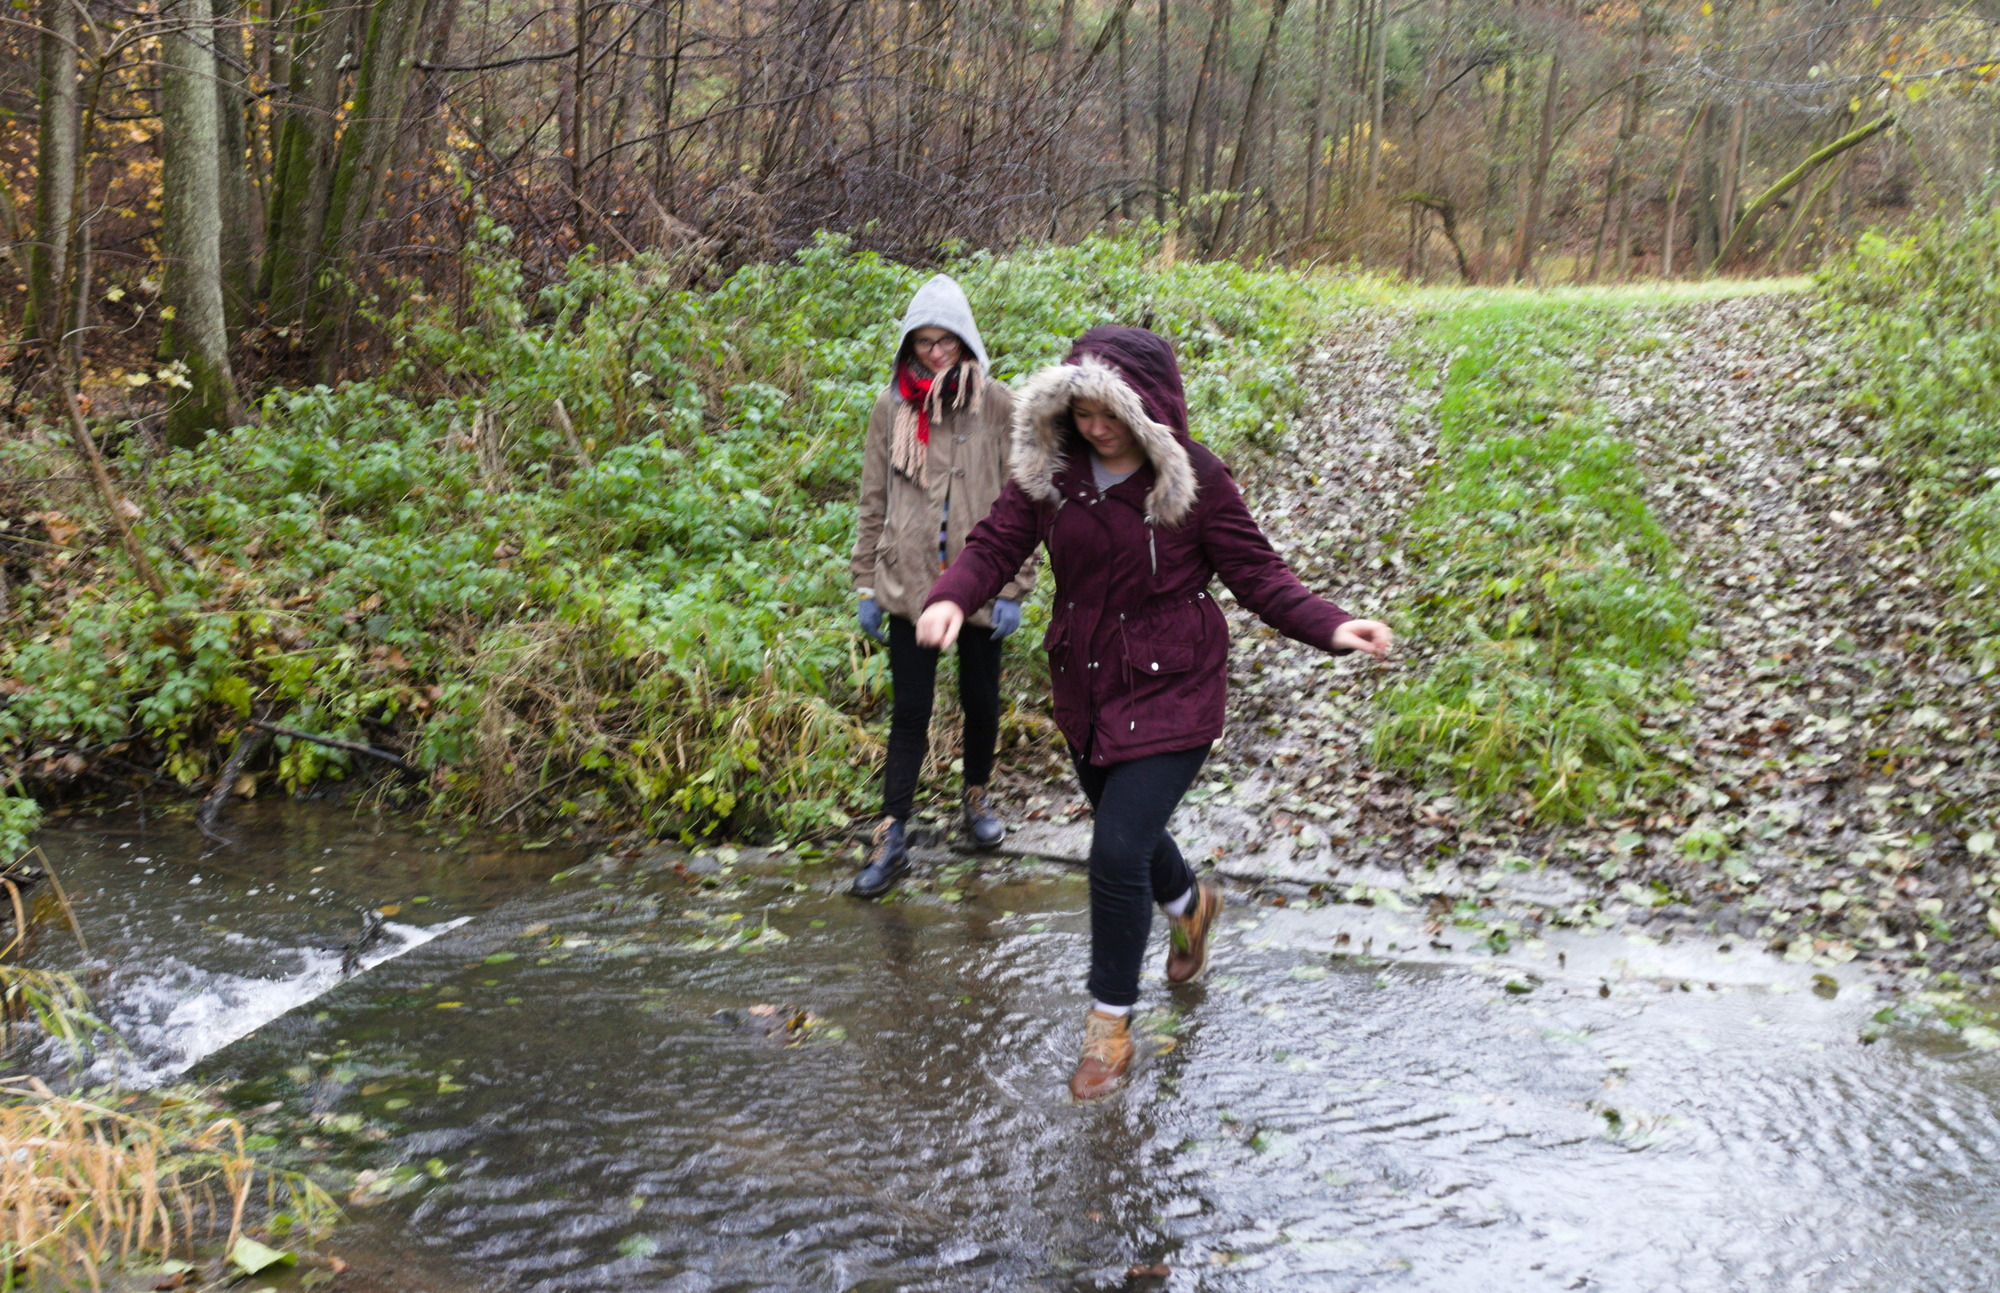
\includegraphics[width=8cm]{img/udo_clanky/hledani_brod.jpg}
\end{center}
\textbf{Prosinec:}

Ještě před novým rokem se hodí mít nalezené vhodné tábořiště a již komunikovat s majitelem. I když někdy to třeba nevyjde…\\
\textbf{Leden, Únor:}

Pokud už tábořiště máme nalezené a majitel souhlasí, je všechno v pořádku a není potřeba se příliš stresovat.\\
Pokud ale tábořiště ještě není, je problém. V takovém případě je potřeba zopakovat všechny předchozí kroky, ale rychleji a efektivněji.\\
\textbf{Březen, Duben:}

Tábor se postupně blíží a vše nabírá konkrétnější rozměry. V průběhu jara se pro jistotu ještě jednou vypraví vybraný uďotým zkontrolovat budoucí tábořiště.\\
\textbf{Květen:}

Konkrétní rozměry jsou ještě konkrétnější a začíná administrativa. Je potřeba řešit například smlouvy související s loukou a odběrem vody z nejbližší vesnice.\\
\textbf{Červen:}

Jde se k praxi a předtáborovému mazlení se se dřevem. Všechny týpiovky zůstávají obvykle na pile v blízkosti bývalého tábořiště. A teď je potřeba je dovézt na to nové. 
Obvykle to zabere jeden celý den, takže je převoz tyčí spíše dvoudenní akcička.\\
\textbf{Červenec:}

Jedeme si postavit svůj tábor, jej!
A tady už přichází vysněná odměna pro tým, který pracoval přes rok: když se na louku postaví několik týpek, hned vypadá úplně jinak.

Někdy se vydaří, a můžeme být na jedné louce dvakrát. To pak odpadá hledání, ale i tak je potřeba někdo, kdo se přes rok o tábořiště zajímá.
Například letošní tábořiště u Ostrovce nám pěkně zavařilo s potokem a pak i rybníkem. Takže pro příští rok jsme kritičtější na ostatní louky a velikost jejich potoků.

\podpis{Koala}

% subsubsection tábor_co_a_jak (end)